\section{Auswertung}
\label{sec:auswertung}

Die in der Auswertung verwendeten Mittelwerte mehrfach gemessener Größen sind gemäß der Gleichung
%
\begin{equation}
    \bar{x}=\frac{1}{n}\sum_{i=1}^n x_i
    \label{eq:mittelwert}
\end{equation}
%
bestimmt.
Die Standardabweichung des Mittelwertes ergibt sich dabei zu
%
\begin{equation}
    \symup{\Delta}\bar{x}=\sqrt{\frac{1}{n(n-1)}\sum_{i=1}^n\left(x_i-\bar{x}\right)^2}.
    \label{eq:standardabweichung}
\end{equation}
%
Resultiert eine Größe über eine Gleichung aus zwei anderen fehlerbehafteten Größen, so berechnet sich der Gesamtfehler nach der Gaußschen Fehlerfortpflanzung zu
%
\begin{equation}
    \symup{\Delta}f(x_1,x_2,...,x_n)=\sqrt{\left(\frac{\partial f}{\partial x_1}\symup{\Delta}x_1\right)^2+\left(\frac{\partial f}{\partial x_2}\symup{\Delta}x_2\right)^2+ \dotsb +\left(\frac{\partial f}{\partial x_n}\symup{\Delta}x_n\right)^2}.
    \label{eq:fehlerfortpflanzung}
\end{equation}
%
Alle in der Auswertung angegebenen Größen sind stets auf die erste signifikante Stelle des Fehlers gerundet.
Setzt sich eine Größe über mehrere Schritte aus anderen Größen zusammen, so wird erst am Ende gerundet, um Fehler zu vermeiden.
Zur Auswertung wird die Programmiersprache \texttt{python (Version 3.4.1)}
mit den Bibliothekserweiterungen \texttt{numpy}, \texttt{scipy} und \texttt{matplotlib} zur Erstellung der Grafiken und linearen Regressionen verwendet.


\subsection{Bestimmung der Grundintensität $I_0$}

Zur Bestimmung der Aktivität der verwendeten Quelle wird zu Beginn eine 
Messung ohne Würfel durchgeführt. Aus dem so aufgenommenen, in 
Abbildung~\ref{fig:nullmessung} dargestellten Spektrum wird eine Rate von 
$I'_0 = 225.4\,\pm\,0.7\:\frac{\text{counts}}{\text{s}}$ bestimmt. Diese 
folgt aus der Messung von $101383$ counts über $\SI{449.8}{\second}$. Der 
statistische Poissonfehler ist aufgrund der großen Anzahl an counts 
$<\SI{1}{\percent}$ und somit vernachlässigbar.

\begin{figure}
    \centering
    \includegraphics[width=0.85\textwidth]{analysis/plots/nullmessung.pdf}
    \caption{Energieverteilung der Nullmessung ohne Würfel im Strahlengang.}
    \label{fig:nullmessung}
\end{figure}

Dieser Wert stellt im weiteren Verlauf der Auswertung den Vergleichswert für 
die Absorptionen dar. Da sich die zu untersuchenden Würfel allerdings in einem 
äußeren Aluminiumgehäuse befinden, wird die zusätzliche Absorption durch 
Messungen leerer Würfel bestimmt. Abbildung~\ref{fig:leermessung} zeigt das 
Spektrum dieser Messung.

\begin{figure}
    \centering
    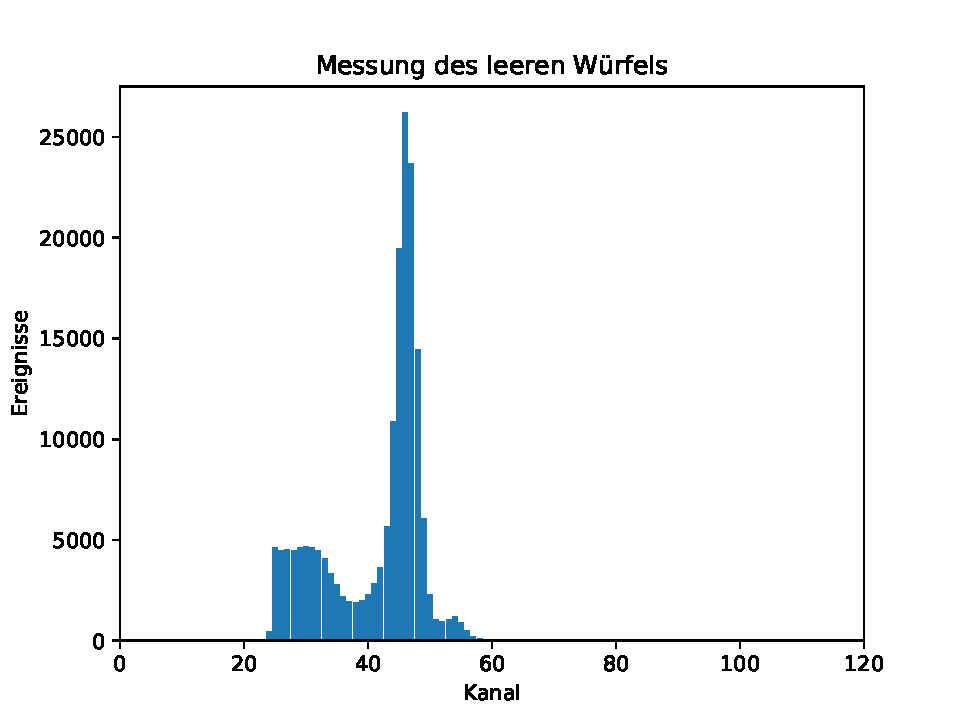
\includegraphics[width=0.85\textwidth]{analysis/plots/leermessung.pdf}
    \caption{Energieverteilung der Leermessung an einem hohlen Aluminiumwürfel.}
    \label{fig:leermessung}
\end{figure}

Um die Raten der Leermessungen für alle 12 später benötigten Strahlrichtungen 
durch den Würfel möglichst exakt zu bestimmen, werden die Messergebnisse der 
einzelnen Richtungen bei gleicher Weglänge durch den Würfel gemittelt. Dazu 
werden die Projektionen 5, 6, 8, 9 und 11 vermessen. So ergibt sich der  
Intensitätsvektor in~\eqref{eq:int} in Reihenfolge der in 
Abbildung~\ref{fig:projektionen} dargestellten Projektionen I1 - I12, sowohl 
wie gemessen als auch gemittelt.

\begin{equation}
	\vec{I}=
	\begin{pmatrix}
		- \\
		- \\
		- \\
		- \\
		200.3\,\pm\,0.6 \\
		215.7\,\pm\,0.7 \\
		- \\
		210.8\,\pm\,0.6 \\
		217.2\,\pm\,0.6 \\
		- \\
		214\,\pm\,0.7 \\
		-
	\end{pmatrix}
	\sfrac{\text{counts}}{\text{s}}\quad
	\vec{\tilde{I}}=
	\begin{pmatrix}
		208\,\pm\,0.6 \\
		208\,\pm\,0.6 \\
		208\,\pm\,0.6 \\
		208\,\pm\,0.6 \\
		208\,\pm\,0.6 \\
		208\,\pm\,0.6 \\
		214\,\pm\,0.7 \\
		214\,\pm\,0.6 \\
		214\,\pm\,0.7 \\
		214\,\pm\,0.7 \\
		214\,\pm\,0.6 \\
		214\,\pm\,0.7
	\end{pmatrix}
    \sfrac{\text{counts}}{\text{s}}
	\label{eq:int}
\end{equation}

\subsection{Auswertung der Würfel aus einheitlichem Material}

Die Würfel 2 und 3 bestehen nach Information des Versuches nur aus Würfeln 
eines Materials. Die Materialien sind Blei (Würfel 2), sowie Messing (Würfel 
3). Daher können die verschiedenen, vermessenen Projektionen im Sinne eines 
überbestimmten Gleichungssystems für eine Mittelung verwendet werden. Ebenso 
kann die Geometriematrix zu einem Vektor in den einzelnen Komponenten 
aufsummiert werden. Es folgt:

\begin{equation}
	A=
	\begin{pmatrix}
		3 \\
		3 \\
		3\cdot\sqrt{2} \\
		3\cdot\sqrt{2}
	\end{pmatrix} \; .
\end{equation}

Diese Matrix beschreibt die Projektionen 2, 5, 8 und 11. Mit Hilfe der 
Methode der kleinsten Quadrate lassen sich nun die Absorptionskoeffizienten 
der einzelnen Materialien bestimmen. Es ergeben sich die in 
Tabelle~\ref{tab:2und3} aufgeführten Ergebnisse.

\begin{table}[htb]
  \centering
  \caption{Aus den verschiedenen Projektionen gemittelte Absorptionskoeffizienten der Würfel 2 und 3.}
  \begin{tabular}{c|
                  S[table-format=1.3(1)]}
    \toprule
    {Objekt} & {Absorptionskoeffizient $\mu$, $\si{\per\centi\meter}$} \\
		\midrule
    Würfel 2 & 0.19(1) \\
    Würfel 3 & 1.04(6) \\
    \bottomrule
  \end{tabular}
  \label{tab:2und3}
\end{table}

\subsection{Auswertung des Würfels unbekannten Aufbaus}

Die Messung des Würfels 5 stellt eine Vermessung eines Würfels mit 
unbekannter innerer Struktur dar. Es ist also weder klar, welche Materialien 
innerhalb des Würfels vorliegen, noch in welcher Verteilung auf die kleinen 
inneren Würfel. Durch die Vermessung des Würfels über alle 12 in 
Abbildung~\ref{fig:projektionen} dargestellten Projektionen lassen sich für 
jeden der 9 inneren Würfel die Absorptionskoeffizienten bestimmen.
Dazu wird hier die folgende Geometriematrix $A$ verwendet.

\begin{equation}
	A=
	\begin{pmatrix}
    1 & 0 & 0 & 1 & 0 & 0 & 1 & 0 & 0 \\
    0 & 1 & 0 & 0 & 1 & 0 & 0 & 1 & 0 \\
    0 & 0 & 1 & 0 & 0 & 1 & 0 & 0 & 1 \\
    1 & 1 & 1 & 0 & 0 & 0 & 0 & 0 & 0 \\
    0 & 0 & 0 & 1 & 1 & 1 & 0 & 0 & 0 \\
    0 & 0 & 0 & 0 & 0 & 0 & 1 & 1 & 1 \\
    0 & \sqrt{2} & 0 & 0 & 0 & \sqrt{2} & 0 & 0 & 0 \\
    \sqrt{2} & 0 & 0 & 0 & \sqrt{2} & 0 & 0 & 0 & \sqrt{2} \\
    0 & 0 & 0 & \sqrt{2} & 0 & 0 & 0 & \sqrt{2} & 0 \\
    0 & 0 & 0 & 0 & 0 & \sqrt{2} & 0 & \sqrt{2} & 0 \\
    0 & 0 & \sqrt{2} & 0 & \sqrt{2} & 0 & \sqrt{2} & 0 & 0 \\
    0 & \sqrt{2} & 0 & \sqrt{2} & 0 & 0 & 0 & 0 & 0
	\end{pmatrix}
\end{equation}

\begin{equation}
	\vec{I}_5=
	\begin{pmatrix}
		118.2\,\pm\,0.5 \\
		19.1\,\pm\,0.2 \\
		115.7\,\pm\,0.6 \\
		46.3\,\pm\,0.4 \\
		45.6\,\pm\,0.4 \\
        115.7\,\pm\,0.6 \\
		62.5\,\pm\,0.4 \\
		28.5\,\pm\,0.3 \\
		131.4\,\pm\,0.6 \\
		123.7\,\pm\,0.6 \\
		29.1\,\pm\,0.4 \\
		77.9\,\pm\,0.7
	\end{pmatrix}
	\sfrac{\text{counts}}{\text{s}}\quad
	\vec{\tilde{I}}=
	\begin{pmatrix}
		0.57\,\pm\,0.09 \\
		2.4\,\pm\,0.2 \\
		0.59\,\pm\,0.09 \\
		1.5\,\pm\,0.1 \\
		1.5\,\pm\,0.2 \\
		0.59\,\pm\,0.09 \\
		1.2\,\pm\,0.1 \\
		2.0\,\pm\,0.2 \\
		0.5\,\pm\,0.1 \\
		0.55\,\pm\,0.09 \\
		2.0\,\pm\,0.2 \\
		1.0\,\pm\,0.1
	\end{pmatrix}
	\label{eq:rate5}
\end{equation}

Die Methode der kleinsten Quadrate liefert dann für die in 
Gleichung~\eqref{eq:rate5} gemessenen Raten und deren normalisierten Logarithmen
die folgenden Absorptionskoeffizienten:

\begin{table}[htb]
  \centering
  \caption{Aus den verschiedenen Projektionen bestimmte Absorptionskoeffizienten der Teilwürfel von Würfel 5.}
  \begin{tabular}{c|
                  S[table-format=1.4(1)]}
    \toprule
    {Teilwürfel} & {Absorptionskoeffizient $\mu$, $\si{\per\centi\meter}$} \\
	\midrule
    1 &  0.35(8)\\
    2 &  0.72(6) \\
    3 &  0.31(8) \\
    4 &  0.06(6) \\
    5 &  1.09(8) \\
    6 &  0.15(6) \\
    7 &  0.14(8) \\
    8 &  0.28(6) \\
    9 &  0.12(8) \\ 
    \bottomrule
  \end{tabular}
  \label{tab:5}
\end{table}